\documentclass[12pt,a4paper,onecolumn,titlepage]{article}
%\documentclass[conference]{IEEEtran} %\Caso queira submeter o artigo para padrão IEEE.

\usepackage[brazil]{babel}
%\usepackage[latin1]{inputenc}
\usepackage[utf8]{inputenc}
\usepackage{graphicx}
\graphicspath{{figuras/}}

\begin{document} %Inicio do documento

\begin{titlepage} %Capa
	
	\vfill
	\begin{center}
	
		{\large \textbf{Faculdade de Ciências e Tecnologia\\Universidade Estadual Paulista\\``Júlio de Mesquita Filho''}} \\[3cm]
		{\large \textbf{Bruno Santos de Lima}}\\
		{\large \textbf{Leandro Ungari Cayres}}\\[4cm]
		{\Large Documento de Requisitos}\\
		{\Large Sistema LearnStation}\\[4cm]

	\hspace{.45\textwidth} %posiciona a minipage
	\begin{minipage}{.5\textwidth}
		\large Disciplina de Engenharia de Software I. Professor Dr. Rogério Eduardo Garcia.\\[0.5cm]
	\end{minipage}

	\vfill
	\vspace{1.5cm}
	
	\large \textbf{Presidente Prudente\\}
	\large \textbf{Abril - 2016}
	
	\end{center}
	
\end{titlepage}
%Fim da capa

%Conteúdo do documento
\section{Introdução}
\label{sect:intro}

\subsection{Propósito do documento de requisitos}

O documento tem como objetivo descrever técnicas e métodos utilizados para desenvolvimento do software, assim como todos os recursos de hardware e software necessários para a elaboração deste, contendo todas as especificações de requisitos necessários. Esta ferramenta não possui um público alvo específico, porém é destinada a todos aqueles que tem interesse em aprender ou transmitir conhecimento.

\subsection{Escopo do produto}

O sistema busca oferecer um compartilhamento de conhecimento entre pessoas, permitindo a interação destas através de um sistema de conversa, interação entre amigos e participação em cursos tanto como professor ou aluno. Além disso, é possível, sendo professor, disponibilizar o seu próprio curso contendo material textual, questionários e até componentes de mídia.

\subsection{Definições, siglas e abreviaturas}

Segue abaixo, a lista de siglas e abreviaturas utilizadas neste documento:
\begin{itemize}
\item RF: Requisito Funcional
\item RNF: Requisito não Funcional
\end{itemize}

\subsection{Visão geral do documento}

Neste documento serão abordados alguns assuntos como divididos a seguir: na Seção \ref{sect:descricao} é apresentado a descrição geral do produto, assim como suas funcionalidades e respectivas restrições bem como o ambiente de execução. A seguir na Seção \ref{sect:requisitos} é descrito o conjunto de todos os requisitos do sistema e do projeto. Por fim a Seção \ref{apoio} temos as informações de apoio.

\section{Descrição geral}
\label{sect:descricao}

\subsection{Perspectiva do Produto}

O sistema utiliza uma máquina de servidor que trabalha diretamente com o banco de dados que mantém dados relativos aos usuários, bem como as interações destes realizadas no sistema, com participação em cursos, em ambos papéis e suas interações com outros usuários.

\subsection{Funções do Produto}


O sistema permite o cadastro de usuários, assim como as interações destes visando o compartilhamento de conhecimentos, através de cursos desenvolvidos por alguns usuários buscando a aprendizagem dos demais.

\begin{figure}[!htb]
  \centering
  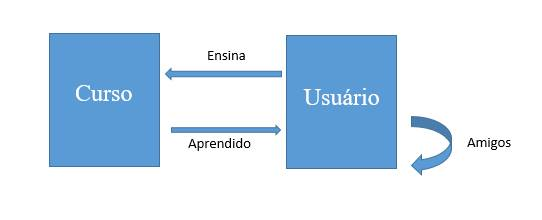
\includegraphics[scale=0.7]{figura1.png}
  \caption{Funcionamento da rede social}
  \label{figRotulo}
\end{figure}


\subsection{Caracteristicas do Usuário}

O usuários do sistema tem como características o interesse em transmitir ou adquirir conhecimentos sobre uma temática especifica, podendo também interagir com os demais usuários afim de potencializar o conhecimento adquirido.

\subsection{Restrições}

O sistema será desenvolvido para uma plataforma web, desta forma podendo ser acessível tanto por desktop ou por dispositivos móveis, sendo que este último tem maiores restrições de hardware e determinados conteúdos relacionados aos cursos podem ter seu desempenho reduzido devido a essas limitações.

Em relação ao restante do projeto este utiliza as recentes tecnologias de desenvolvimento web, logo usuários que possuam navegadores desatualizados poderão enfrentar algumas dificuldades.

\subsection{Suposições e Dependências}

Este software não possui nenhuma limitação quanto ao sistema operativo ou hardware.

\section{Requisitos Específicos}
\label{sect:requisitos}

%\subsection{Interfaces Externas} Poderia usar um sistema externo para criptografar contas de usuarios.


\subsection{Requisitos Funcionais}

%Acho que não precisa separar por tópicos específicos, a numeração basta como no exemplo do slide dele
%RF. 1: Usuário.

%RF. 1.1: Manter Usuário.

RF. 1.1: Registrar dados do usuário após o cadastro no sistema. (E)

RF. 1.2: Busca e listagem de usuários. (E)

RF. 1.3: Exibir perfil de usuário que foi buscado ou de usuário, que é professor de um determinado curso.

RF. 1.4: Enviar e responder solicitação de amizade. (E)

RF. 1.5: Exclusão de amizade. (E)

RF. 1.6: Busca e listagem de cursos. (E)

RF. 1.7: Inscrição em Curso. (E)

RF. 1.8: Cancelamento de Inscrição em Curso. (E)

RF. 1.9: Criar Curso. (E)

RF. 1.10: Avaliar qualidade de cursos. (E)

%Pode tirar o 1.13 é apenas algo que pensei, mas talvez eu tenha viajado um pouco.
%Não é viagem, não este mecanismo não será externo mas sim interno, pesquisar por md5 php
RF. 1.11: Realizar criptografia da senha de usuários. (O)

RF. 1.12: Enviar e receber mensagens para amigo por meio de conversa. (E)

RF. 1.13: Notificação de recebimento de uma mensagem de um amigo no chat. (E)

RF. 1.14: Notificações de informação, na forma de aviso de aulas novas inseridas no curso em que está inscrito ou de solicitação de amizade. (E)

%RF. 2: Curso.
RF. 2.1: Manter Aula. (E)

RF. 2.1: Exibir perfil do curso. (E)


%RF. 3: Aula.

%Mudaria o 3.1 e o 3.2 Anexar materiais das aulas e na descrição do requisito informar os tipos de materiais.
RF. 3.1: Anexo Documentos de Texto. (E)

RF. 3.2: Anexo de Elementos de Mídia. (E)

RF. 3.3: Manter Exercicíos. (E)

RF. 3.4: Exibir informação da Aula. (E)


\subsection{Requisitos Não Funcionais}

%Abaixo apenas listei algumas ideia para os requisitos não funcionais.


RNF. 1: O sistema será desenvolvido para a plataforma web utilizando como linguagem de programação o PHP, além de linguagem de marcação HTML, CSS, assim como utilizando JavaScript.\\

RNF. 2: Para utilizar o sistema basta utilizar um software para navegação na internet e utilizar um endereço para comunicação com o servidor em que o sistema está rodando e assim começar a utilizar a rede social LearnStation.\\

RNF. 3: Para o armazenamento dos dados será utilizado o Sistema de Gerenciamento de Banco de Dados MySQL.\\

%Esse aqui foi viajado
%RNF: 3: O sistema está em funcionamento em dois servidores um deles sendo o principal e o outro o secundario para caso ocorra %algum problema com o servidor principal o sistma ainda possa continuar em funcionamento.\\

%Talvez eu tenha viajado um pouco quanto a isso.
%RNF: 4: A rede social vai utilizar um sistema externo de criptografia para realização de login e logout por parte dos usuarios %afim de prover uma maior segurança.\\

%\subsection{Requisitos Desempenho}
%\subsection{Requisitos Lógicos de Banco de Dados}
%\subsection{Restrições de Projeto}
%\subsection{Atributo do Sistema de Software}



\subsection{Organização}
\section{Informações de Apoio}
\label{apoio}

\section{Índice}
\label{sect:indice}

\section{Apêndices}
\label{sect:apendices}

%Fim do conteúdo do documento
%referencias - estilos: http://www.cs.stir.ac.uk/~kjt/software/latex/showbst.html
%\bibliographystyle{acm}
%\bibliography{referencias}

\end{document} %Fim do documento
